\documentclass[11pt,a4paper,oneside]{report}
\usepackage{amsmath,amssymb,calc,ifthen}
\usepackage{float}
%\usepackage{cancel}
\usepackage[table,usenames,dvipsnames]{xcolor} % for coloured cells in tables
\usepackage{tikz}
% Allows us to click on links and references!
\usepackage{hyperref}
\usepackage{url}
\hypersetup{
colorlinks,
citecolor=black,
filecolor=black,
linkcolor=black,
urlcolor=black
}
% Nice package for plotting graphs
% See excellent guide:
% http://www.tug.org/TUGboat/tb31-1/tb97wright-pgfplots.pdf
\usetikzlibrary{plotmarks,shapes}
\usepackage{amsmath,graphicx}
\usepackage{epstopdf}
\usepackage{caption}
\usepackage{subcaption}
% highlight - useful for TODOs and similar
\usepackage{color}
\newcommand{\hilight}[1]{\colorbox{yellow}{#1}}
\newcommand\ci{\perp\!\!\!\perp} % perpendicular sign
\newcommand*\rfrac[2]{{}^{#1}\!/_{#2}} % diagonal fraction
\newcommand\SLASH{\char`\\}
\usepackage{listings}
% margin size
\usepackage[margin=0.9in]{geometry}

\usepackage{titlesec} % reduce spacing after subsections

\titlespacing\subsection{0pt}{4pt plus 4pt minus 2pt}{4pt plus 2pt minus 2pt}


\tikzstyle{state}=[circle,thick,draw=black, align=center, minimum size=2.1cm,
inner sep=0]
\tikzstyle{vertex}=[circle,thick,draw=black]
\tikzstyle{terminal}=[rectangle,thick,draw=black]
\tikzstyle{edge} = [draw,thick]
\tikzstyle{lo} = [edge,dotted]
\tikzstyle{hi} = [edge]
\tikzstyle{trans} = [edge,->]
\definecolor{mygreen}{rgb}{0,0.6,0}
\definecolor{mygray}{rgb}{0.5,0.5,0.5}
\definecolor{mymauve}{rgb}{0.58,0,0.82}
\DeclareMathOperator*{\argmin}{arg\,min}
\DeclareMathOperator*{\argmax}{arg\,max}
\lstset{ %
backgroundcolor=\color{white}, % choose the background color; you must add
%\usepackage{color} or \usepackage{xcolor}
basicstyle=\footnotesize, % the size of the fonts that are used for the
%code
breakatwhitespace=false, % sets if automatic breaks should only happen
%at whitespace
breaklines=true, % sets automatic line breaking
captionpos=b, % sets the caption-position to bottom
commentstyle=\color{mygreen}, % comment style
deletekeywords={...}, % if you want to delete keywords from the
%given language
escapeinside={\%*}{*)}, % if you want to add LaTeX within your code
extendedchars=true, % lets you use non-ASCII characters; for
%8-bits encodings only, does not work with UTF-8
frame=single, % adds a frame around the code
keepspaces=true, % keeps spaces in text, useful for keeping
%indentation of code (possibly needs columns=flexible)
keywordstyle=\color{blue}, % keyword style
language=Octave, % the language of the code
morekeywords={*,...}, % if you want to add more keywords to the set
numbers=left, % where to put the line-numbers; possible
%values are (none, left, right)
numbersep=5pt, % how far the line-numbers are from the code
numberstyle=\tiny\color{mygray}, % the style that is used for the line-numbers
rulecolor=\color{black}, % if not set, the frame-color may be changed
%on line-breaks within not-black text (e.g. comments (green here))
showspaces=false, % show spaces everywhere adding particular
%underscores; it overrides 'showstringspaces'
showstringspaces=false, % underline spaces within strings only
showtabs=false, % show tabs within strings adding particular
%underscores
stepnumber=2, % the step between two line-numbers. If it's
%1, each line will be numbered
stringstyle=\color{mymauve}, % string literal style
tabsize=2, % sets default tabsize to 2 spaces
title=\lstname % show the filename of files included with
%\lstinputlisting; also try caption instead of title
}
\title{Computational Modelling for Biomedical Imaging - Coursework 1}
\author{
Razvan Valentin Marinescu\\
Student Number: 14060166\\
\texttt{razvan.marinescu.14@ucl.ac.uk}
}
\begin{document}
\belowdisplayskip=12pt plus 3pt minus 9pt
\belowdisplayshortskip=7pt plus 3pt minus 4pt

\begin{titlepage}
\begin{center}

% Upper part of the page. The '~' is needed because \\
% only works if a paragraph has started.

\includegraphics[width=0.2\textwidth]{ucl-logo2}~\\[1cm]

\textsc{\LARGE University College London}\\[1.5cm]

%\textsc{\Large MRes Project Plan}\\[0.5cm]

\newcommand{\HRule}{\rule{\linewidth}{0.5mm}}

% Title
\HRule \\[0.4cm]
{ \LARGE Computational Modelling in Biomedical Imaging - Coursework 2 \\[0.4cm] }

\HRule \\[1.5cm]

% Author and supervisor
\begin{minipage}{0.4\textwidth}
%\begin{flushleft} \large
\begin{center}
\textsc{\large
\emph{Author:}\\
R\u{a}zvan Valentin \textsc{Marinescu}}\\
\href{razvan.marinescu.14@ucl.ac.uk}{razvan.marinescu.14@ucl.ac.uk}\\
%\end{flushleft}

\end{center}
\end{minipage}

\vfill
\vfill
\vfill
\textsc{\large
EPSRC Centre for Doctoral Training in Medical Imaging\\ University College London}

\vfill

% Bottom of the page
{\large \today}

\end{center}
\end{titlepage}



\rowcolors{1}{gray!25}{white}

\subsection*{Part 1 - Q1}
\noindent \large{\textbf{(a)}} \begin{tabular}{c | c | c | c | c}
Sample & True mean & Sample mean & True std. dev. & Sample std. dev.\\
sample 1 & 1 & 0.9848 & 0.25 & 0.2842\\
sample 2 & 1.5 & 1.4944 & 0.25 & 0.2281\\
\end{tabular}\\

The new values are as expected, lying within a 0.04 tolerance level.\\

\noindent \large{\textbf{(b)}} The t-test results in a t-statistic of -6.9923, rejecting the null hypothesis with a p-value of 7.55e-09 which is very low. We are very confident the two samples were generated from distributions with different means, which is indeed the case (means of 1 and 1.5).

\rowcolors{1}{}{}
\noindent \large{\textbf{(c)}} \textbf{i.} $X = \begin{pmatrix}
1 & \dots & 1 & 0 & \dots & 0\\
0 & \dots & 0 & 1 & \dots & 1\\

\end{pmatrix}^T$ where $range(X) = 50 \times 2$ and $dim(X) = 2$ because $X$ is made of two column vectors that are linearly independent.\\


\textbf{ii.} $Y = X\beta \to X^TY = X^TX\beta \to (X^TX)^{-1}X^TY = \beta \to X(X^TX)^{-1}X^TY = X\beta$. Since $MY = X\beta$, we deduce $M = X(X^TX)^{-1}X^T$. In our case $M = 
0.04 * \begin{pmatrix}
\mathbb{I}_N & 0\\
0 & \mathbb{I}_N
\end{pmatrix}
$
where $\mathbb{I}_N$ is an $N \times N$ matrix full of 1's (not to be confused with the identity matrix $I_n$).\\
                          
\textbf{iii.} $\hat{Y} = MY = [ 0.9848 \dots 0.9848 \; 1.4944 \dots 1.4944]^T$ and $\hat{e} = (I-M)Y$. The cosine between the vectors is almost zero (-4.1352e-16) which means that the vectors are perpendicular. This is what we expected, since the column space and error space are orthogonal.\\

\textbf{iv.} We know that $Y = X\beta$. Pre-multiplying by $X^T$ gives $X^TY = X^TX\beta$. Now matrix $X^TX$ is a square matrix and can normally be inverted. We therefore further pre-multiply by $(X^TX)^{-1}$ and get $(X^TX)^{-1}X^TY = \beta$, the model parameters. For our problem we get the estimated parameters $\beta = [0.9848, 1.4944]$, which are very close to the ground truth values of $[1, 1.5]$\\

\textbf{v.} $$\hat{\sigma}^2 = \frac{\hat{e}^T\hat{e}}{n - dim(X)} = \frac{(Y - X\hat{\beta})^T(Y - X\hat{\beta})}{n - dim(X)}$$. This is called the \emph{Mean Squared Error} because it is an unbiased estimate of the error in the prediction. The upper term $(Y - X\hat{\beta})^T(Y - X\hat{\beta})$ is the sum of squared differenced between the observations and the predicted values. This is then divided by the number of degrees of freedom, which is $N - 2$ in our case. For our error vector we get $\hat{\sigma}^2 = 0.0664$.\\

\textbf{vi.} $S_{\hat{\beta}} = \hat{\sigma}^2(X^TX)^{-1} = \begin{pmatrix}
0.0027 & 0\\
0 & 0.0027
\end{pmatrix}$. From $S_{\hat{\beta}}$ we can calculate $std(\beta_1) = \sqrt{Sb(1,1)} = 0.0515$. Similarly we get  $std(\beta_2) = \sqrt{S_{\hat{\beta}}(2,2)} = 0.0515$. The parameters are independent from each other because the covariance (off-diagonal) terms in $S_b$ are both zero.\\

\textbf{vii.} $C = [1, -1]^T \to C'\beta = \beta_1 - \beta_2 = 0$. By setting $\beta_1 = \beta_2 = \gamma$ we then solve $Y = X_0\gamma = XU\gamma$ so it must be the case that $\beta = U\gamma$. Solving this for our conditions gives $U = [1, 1]^T$. Then the reduced model $X_0 = XU = [1 \dots 1]^T $ where the length of $X_0$ is 50. \\


\textbf{viii.} If $\hat{Y}$ and $\hat{Y_c}$ are the predicted values using the full and constrained models respectively, then $\hat{Y}_{\perp c} = \hat{Y} - \hat{Y_c}$ is the additional error. For our data we get $|\hat{Y_{\perp c}}| = 1.8017$. Using the MSE we got from (v), we get 

$$F = \frac{|\hat{Y}_{\perp c}|^2 / r}{|\hat{e}|^2 / (N - p)} = 48.89$$

Since $F > 3.68$, we reject $H_0$ at $a = 0.05$ confidence level (i.e. the two samples come from different groups).\\

\textbf{ix.} The t-statistic is -6.9923 and is exactly the same as the one calculated in point b). In our example it is also the case that $t^2 = F$.\\

\textbf{x. } The model parameters represent the \emph{estimated values} for the means of the distributions that we used to sample the data from. In our case we get $\hat{\beta} = [0.9848, 1.4944]$ which are close to the true values of $\beta = [1, 1.5]$. \\

\textbf{xi. } $e_c = M e = [-0.0152 \dots -0.0152 \; -0.0056 \dots -0.0056 ]$ where elements from each part of the array are exactly the differece between $\hat{\beta} - \beta = [-0.0152 \; -0.0056]$. $e_c$ represents the error component that doesn't come from noise, but from the wrong estimates of $\hat{\beta}$ that are not equal to the true $\beta$. \\

\textbf{xii. } $e_{error} = (I - M) e = (I - M) (Y - X\beta) = (I - M)Y - (I - M)X\beta = \hat{e} - 0 = \hat{e}$ because $(I-M)$ and $X\beta$ are orthogonal. Numerical values in our example confirm that $e_{error} = \hat{e}$, which means that the projection of the ground truth error $e$ onto the error space is the same as the measured error $\hat{e}$. This suggests that the measured error $\hat{e}$ is always smaller that the true error $e$. \\

\noindent \large{\textbf{(d)}} \textbf{i. } $X = \begin{pmatrix}
1 & \dots & 1 & 1 & \dots & 1\\
1 & \dots & 1 & 0 & \dots & 0\\
0 & \dots & 0 & 1 & \dots & 1\\
\end{pmatrix}^T$  where $range(X) = 50 \times 3$ and $dim(X) = 2$ because vectors in $X$ are linearly dependent $X_1 = X_2 + X_3$, so at most two vectors are linearly independent. \\

\textbf{ii. } $C = [0, 1, -1]^T \to \beta_1 = \beta_2 \to U = null(C^T) = \begin{pmatrix}
-0.707 & 0.707\\
0.5 & 0.5\\
0.5 & 0.5\\
\end{pmatrix} \to X_0 = X U = \begin{pmatrix}
-0.207 & 1.207\\
\vdots & \vdots\\
-0.207 & 1.207\\
\end{pmatrix}$\\

\textbf{iii. } $t = -6.9923$, which is the same value obtained with the previous GLM. \\

\textbf{iv. } $\beta_0$ models the constant factor for both groups, $\beta_1$ models the first group and $\beta_2$ models the second group. However, by removing one of the parameters we still get the same fit, so one of them is redundant ($dim(X) = 2$). Our fit gives the following parameters $\beta = [0.826 0.158 0.667]^T$, which is a good fit since $\beta_0 + \beta_1 = 0.9848 \approx 1$ and $\beta_0 + \beta_2 = 1.4944 \approx 1.5$, where $[1, 1.5]$ are the true means. 

\noindent \large{\textbf{(e)}} \textbf{i. } $X = \begin{pmatrix}
1 & \dots & 1 & 1 & \dots & 1\\
1 & \dots & 1 & 0 & \dots & 0\\
\end{pmatrix}^T$ where $range(X) = 50 \times 2$ and $dim(X) = 2$ because $X$ has two vectors that are linearly independent.

\textbf{ii. } $C = [0, 1]^T \to \beta_0 = 0 \to U = null(C^T) = [-1, 0]^T \to X_0 = X U = \begin{pmatrix}
-1\\
\vdots\\
-1\\
\end{pmatrix}$

\textbf{iii. } $t = -6.9923$, which is the same value obtained with the previous GLM's. \\

\textbf{iv. } $\beta_0$ models a constant term for both groups while $\beta_1$ models only the first group. This GLM gives $\hat{\beta} = [1.4944 -0.5096]$, and it is the case that $\beta_0 + \beta_1 = 0.9848 \approx 1 = \mu_0$ and $\beta_0 = 1.4944 \approx 1.5 = \mu_1$, suggesting the fit is very good.\\

\noindent \large{\textbf{(f)}} We cannot test that the samples have different means with the model $Y=X_0\beta_0$ because this model already assumes that all samples have the same mean. In order to test that the two groups have different means one needs a more complex model.\\

\subsection*{Part 1 - Q2}

\noindent \large{\textbf{(a)}} \textbf{i. } $t = -6.9918$, which is different from the t-statistic obtained in question 1. Although the difference is quite small, for a different random number seed, a bigger $\Delta t$ can be observed (see \texttt{p12testT.m}). 

\noindent \large{\textbf{(b)}} \textbf{i. } $X = \begin{pmatrix}
1 & \dots & 1 & 1 & \dots & 1\\
1 & \dots & 1 & 0 & \dots & 0\\
& I_n & & & I_n &\\
\end{pmatrix}^T$  where $range(X) = 50 \times 27$ and $I_n$ is the identity matrix of dimensions $n \times n$. Moreover, rank($X$) = 26 because $X_0 = X_2 + X_3 + \dots + X_{27}$.

\textbf{ii. } $C = [0, 1, 0, \dots, 0]^T \to$ the reduced model $X_0 = \begin{pmatrix}
1 & \dots & 1 & 1 & \dots & 1\\
& I_n & & & I_n &\\
\end{pmatrix}^T$\\

\textbf{iii. }  $t = -6.9918$, which is the same answer as in part (a).\\

\subsection*{Part 2 - Q1}

\noindent \large{\textbf{(a)}} $t = 5.2295$ and $p=2.114e-04$. $H_0$ is rejected at the 5\% significance level (the two samples have different means).\\

\noindent \large{\textbf{(b)}} $p=3.33e-04 = 1/3003$ which is close to the original p-value of $2.11e-04$. However, a better resolution cannot be obtained because the number of permutations is 3003 and with our data only one t-statistic was bigger than the original t-value. The empirical distribution of the t-statistic is plotted in figure \ref{p21b}.\\

\noindent \large{\textbf{(c)}} $p=3.33e-04 = 1/3003$ which is the same value as in part (b). The empirical distribution of the difference between the means is plotted in figure \ref{p21c}.\\

\noindent \large{\textbf{(d)}} \textbf{i. } $p = 0$ when 1000 runs are used because no $t$-values bigger than the original $t$ are found. Increasing the number of runs to 10,000 gives a $p= 3e-04$, which is closer to the original value.

\textbf{ii. } The approximated $p$-value is close to the true $p$-value in points (b) and (c), its accuracy increasing with the number of runs.

\textbf{iii. } There are 159 duplicates in our set of permutations, but removing them doesn't have a big effect on the p-value computation, which for 10,000 runs would be $p=3.44e-04$\\

\subsection*{Part 2 - Q2}

\noindent \large{\textbf{(a)}} Maximum $t$-statistic $max(t) = 6.5294$, computed using the GLM: $Y = X_1 \beta_1 + X_2 \beta_2 + e$.

\noindent \large{\textbf{(b)}} See figure \ref{p22b} for a distribution of the maximum $t$ statistic.

\noindent \large{\textbf{(c)}} The multiple-comparisons-corrected $p$-value is $p = 0.0918$ so we don't reject $H_0$ at 5\% significance level: the two groups of images might have the same mean.

\noindent \large{\textbf{(d)}} The maximum $t$-statistic threshold correspondong to a $p$-value of 5\% is $t = 6.9379$.

\clearpage

\section*{Appendix}

\begin{figure}[H]
\centering
 \includegraphics[scale = 0.7]{figures/p21_b.eps}
 \caption{Empirical distribution of the t-statistic in part 2 - question 1. b). The distribution is centered around zero.}
 \label{p21b}
\end{figure}

\begin{figure}[H]
\centering
 \includegraphics[scale = 0.7]{figures/p21_c.eps}
 \caption{Empirical distribution of the t-statistic in part 2 - question 1. c). The distribution is centered around zero.}
 \label{p21c}
\end{figure}

\begin{figure}[H]
\centering
 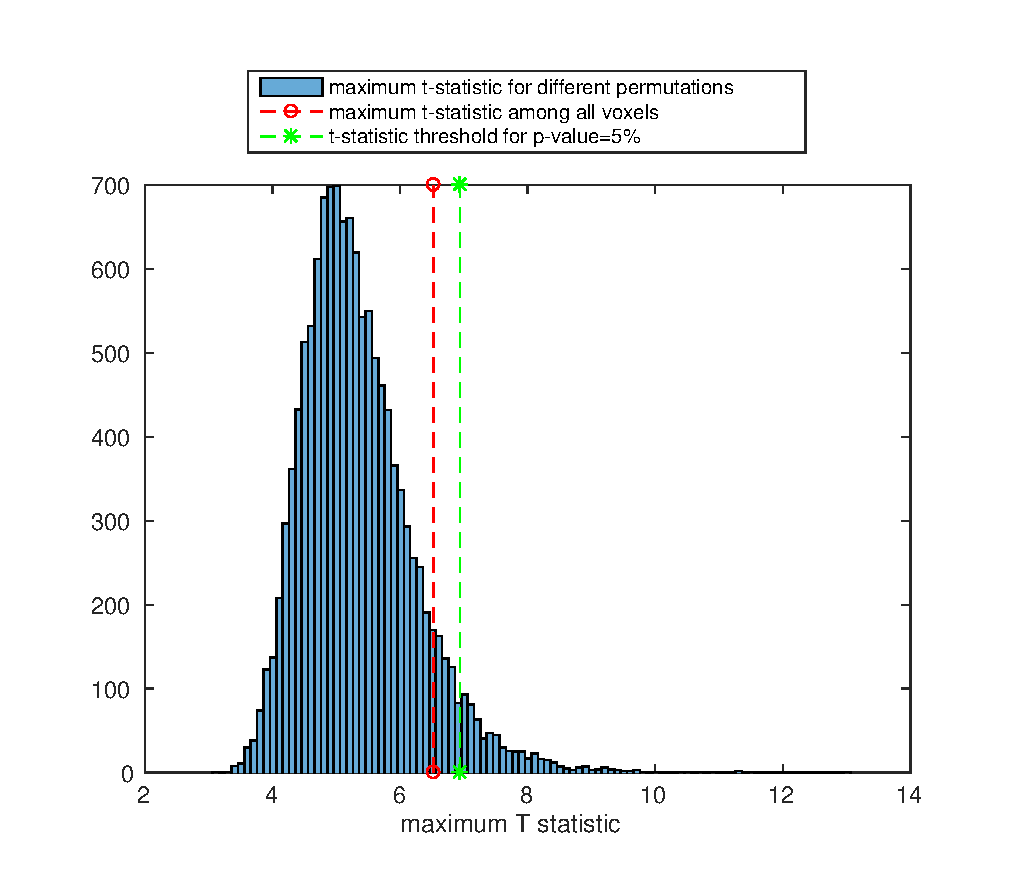
\includegraphics[scale = 0.9]{figures/p22_b.eps}
 \caption{Empirical distribution of the maximum t-statistic for the 40x40x40 images in part two - question two. The t-values are all positive because only the maximum t-statistics across all voxels are plotted. Plotted in red is the maximum t-statistic among all voxels (part a, $max(t) = 6.5294$), while in green is the t-statistic threshold for p-value = 5\% (part (d), $thresh(t) = 6.9379$). The distribution is skewed to the left.}
 \label{p22b}
\end{figure}



\end{document}






















